\section{Macchina a stati finiti}
Il firmware implementato è stato formalizzato tramite una macchina a stati finiti (FSM). Un'automa a stati finiti è un modello matematico con cui è possibile descrivere in modo preciso e sintetico il comportamento di un sistema tramite un numero finito di stati, che rappresentano le condizioni operative nelle quali esso si può trovare. Il passaggio da uno stato all'altro avviene in seguito al verificarsi di particolari eventi e condizioni, che definiscono le \textit{funzioni di transizione}. Una caratteristica fondamentale delle FSM è rappresentata dalla necessità di garantire l'unicità dello stato che in un certo istante di tempo è attivo\todo{da rileggere}. Per questo motivo, è sempre possibile sapere con esattezza lo stato in cui si trova la macchina. Inoltre, è consentito effettuare solo una transizione alla volta. Le transizioni possibili da un particolare stato devono quindi essere mutuamente esclusive.
L'utilizzo di una macchina a numero finito di stai può essere adatto sia per la progettazione di un sistema sia per la descrizione di uno esistente. In particolare, è possibile modellare sistemi che sono:
\begin{itemize}
	\item dinamici, che quindi evolvono cambiando stato nel tempo;
	\item discreti, cioè che le variabili in ingresso e gli stati del sistema si possono rappresentare con valori discreti;
	\item a simboli finiti, cioè che il numero di variabili in ingresso e gli stati può essere espresso con un numeri finito;
\end{itemize}
Una macchina a stati può essere rappresentata attraverso un grafo, in cui i nodi identificano gli stati e gli archi rappresentano le transizioni causate da eventi. 

Il firmware realizzato per questo progetto è stato implementato, con le opportune modifiche, sia per l'acquisizione dei dati con il sensore MAX86916 sia con l'integrato MAXM86161. Sono stati identificati i seguenti stati:
\begin{enumerate}
	\setcounter{enumi}{-1}
	\item Start-up
	\item Idle
	\item Stream
	\item Error
\end{enumerate}
La figura \ref{fig:FSM} mostra il grafo della macchina a stati finiti implementata.
Nella figura \ref{fig:FSM} è stato riportato il grafico che riassume il comportamento della macchina a stati implementata.
\begin{figure}[tb]
	\centering
	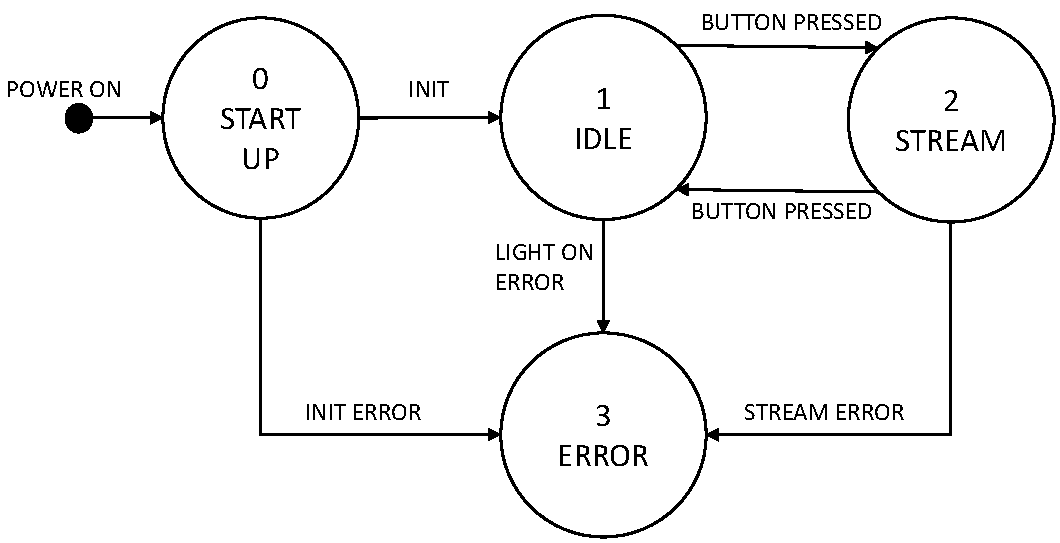
\includegraphics[width=0.6\linewidth]{ImageFiles/Macchina a stati finiti/FSM}
	\caption{Macchina a stati finiti del firmware delle due board progettate.}
	\label{fig:FSM}
\end{figure}
\paragraph{Start-up}
\paragraph{Idle}
\paragraph{Stream}
\paragraph{Error}

\clearpage